\section{Introducción}

\subsection{El lenguaje Gobstones}

Gobstones\cite{Gobstones} [TODO: hablar sobre gobstones]

\subsection{Editores Proyectivos}

El término Editor Proyectivo fue acuñado por Martin Fowler en el año 2005\cite{Fowler}, al intentar plantear un ambiente de desarrollo donde el programador pudiera expresar sus ideas en términos de conceptos en lugar de texto. Lo que vemos como texto pasaría entonces a constituir una representación editable del concepto al que hace referencia (y al cual Fowler llama \textit{representación abstracta}).

De esta manera, los conceptos del lenguaje son el dominio de los editores proyectivos, y decimos que un programa es una \textit{representación abstracta} construida utilizando dichos conceptos. Para modificar esta representación el programador interactúa con una interfaz de usuario, llamada \textit{representación editable}, sobre la cual la \textit{representación abstracta} se \textit{proyecta} en forma de texto\cite{voelter2014projectional}. 

\begin{wrapfigure}[10]{r}{0.5\textwidth}
  \begin{center}
    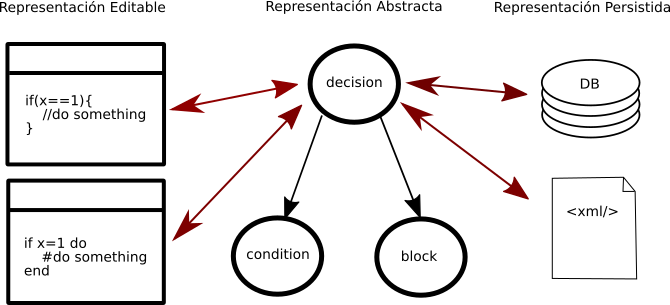
\includegraphics[width=0.5\textwidth,keepaspectratio]{assets/projectional-editor.png}
    \caption{Representaciones de un programa en un editor proyectivo}
  \end{center}
\end{wrapfigure}


A su vez, la \textit{representación abstracta} puede persistirse de diferentes maneras a diferentes soportes, con lo cual se introduce la idea de \textit{representación persistida} para hablar del formato en que guardará el programa, ya sea en una base de datos, un archivo binario, un texto con formato XML, etc.


Esto tiene varias consecuencias:
\begin{itemize}
  \item Deja de necesitarse un parser para el lenguaje, volviéndolo más sencillo de extender.
  \item El programador trabaja más cerca de los conceptos que quiere expresar.
  \item Reduce drásticamente los posibles errores de sintaxis.
  \item El editor trabaja directamente con las instancias de los conceptos, con lo cual:
  \begin{itemize}
    \item es más sencillo analizar el programa
    \item se simplifica la construcción de herramientas (ej: refactors, migrado de versiones de lenguaje, intentions, etc)
    \item se mejora la performance del editor al eliminarse la etapa de parseo.
  \end{itemize}
\end{itemize}


\subsection{MPS Workbench}

MPS (Meta programming System)\cite{MPS} es un ambiente de trabajo orientado al desarrollo de lenguajes específicos de dominio, de la empresa JetBrains, basado en las ideas de Fowler; hoy en día se posiciona como uno de los referentes más importantes en editores proyectivos\cite{LanguageModularity}. 
Entre los productos desarrollados utilizando MPS se encuentran \textit{MetaR} \cite{MetaR}, un ambiente especializado en biomedicina computacional, y \textit{mbeddr} \cite{mbeddr}, un ambiente orientado a software embebido.

\section{Motivación}

En el libro \textit{"Las bases conceptuales de la Programación. Una nueva forma de aprender a programar"}\cite{Gobstones} se presenta una secuencia didáctica bien detallada junto con el entorno \textit{PyGobstones}\cite{PyGobstones}, pero notamos que en el marco de una adopción cada vez mayor de esta didáctica es necesario:

\begin{itemize}
  \item disponer de un ambiente que sea fácilmente extensible y posea una arquitectura que agilice la colaboración de la comunidad de Gobstones.
  \item que el ambiente sea un refuerzo de la se secuencia didáctica, y no sólo una herramienta de edición.
  \item utilizar tecnologías que posean un buen soporte y comunidad.
  \item que el entorno sea sencillo de instalar
\end{itemize}


\section{Propuesta}

Se propone utilizar \textit{MPS Workbench} para implementar un \textit{Entorno Integral de Aprendizaje}, supliendo las necesidades antes mencionadas, siendo que:

\begin{itemize}
  \item soporta tanto extensión de lenguaje como extensión del entorno mediante la creación de plugins que pueden no depender entre sí.
  \item los features de lenguaje pueden ser activados y desactivados durante el uso del entorno para cumplir con la secuencia didáctica.
  \item es soportado por JetBrains, uno de los líderes mundiales en desarrollo de entornos de programación.
  \item el entorno sólo necesita Java Runtime Environment (siendo que se trabajará sobre la implementación de un intérprete Gobstones, con lo cual se vuelve innecesario contar con un compilador).
\end{itemize}

A su vez, la naturaleza proyectiva del entorno le permite al alumno concentrarse en el concepto que desea expresar al evitarle errores comunes de sintaxis. Además, el programa siempre se presenta al alumno con un formato estándar (bien indentado, secciones organizadas, etc), ayudándolo a incorporar más rápidamente estas buenas prácticas al reconocerlas como algo natural. Esto es así porque al principio el alumno no posee una noción de estilos \textit{correctos}, sino que se va formando a medida que es expuesto a ellos.

En particular, esta implementación busca:
\begin{itemize}
  \item que el lenguaje refuerce la necesidad de buenos comentarios y la especificación del propósito y precondición de funciones y procedimientos
  \item el uso de estilos sutiles que faciliten el reconocimiento estructuras repetidas; por ejemplo, coloreando nodos similares al que se encuentre debajo del cursor. Esto se vuelve útil a la hora de enseñar determinados conceptos, como la parametrización de procedimientos.
\end{itemize}

Todo esto siguiendo la filosofía de Gobstones y buscando mantener las virtudes de la implementación original (identidad gráfica, multiplataforma, interfaz de usuario minimalista, etc).

\section{Plan de trabajo}

[TODO: transcribir los sprints planificados en waffle]
